\documentclass[conference,compsoc]{IEEEtran}
\usepackage{cite}
\usepackage{listings}
\usepackage{blindtext}
\usepackage{enumitem}
\usepackage{float}
% for coding highlight
\usepackage{graphicx}
\usepackage[colorlinks=true,urlcolor=blue]{hyperref}
\usepackage{amsmath, amsthm, amssymb}
\usepackage{subfloat}
\usepackage{ulem}
\usepackage{indentfirst}
\usepackage{booktabs}
\usepackage{wrapfig,lipsum,booktabs}
\usepackage{array}
\newcommand{\subparagraph}{}
\newcolumntype{C}[1]{>{\centering\let\newline\\\arraybackslash\hspace{0pt}}m{#1}}

\begin{document}
\title{
	Deep Learning Final Project Report \\
	Passenger Screening Algorithm Challenge \\
}


% author names and affiliations
% use a multiple column layout for up to three different
% affiliations
\author{
	\IEEEauthorblockN{Yuyang Rong}
	\IEEEauthorblockA{
		School of Information Science and Technology \\
		ShanghaiTech University \\
		Student ID: 69850764 \\
	}
\and
	\IEEEauthorblockN{Peng Ding}
	\IEEEauthorblockA{
		School of Information Science and Technology \\
		ShanghaiTech University \\
		Student ID: 79406120 \\
	}
}

\maketitle

\begin{abstract}
The safety issue has always been a major concern since the day that aviation was civilianized. Dectecting whether passengers are carrying any prohibited items is one of the key steps before passenger board the plane. Conventionally, passengers are required to be screened and physically examined by TSA staffs. Such procedure takes time and effort to operate, without guaranteeing the accuracy of checking. Whereas complaints call upon the invasion of personal privacy. With all these being considered, people rarely consider the traditional security check as a satisfactory experience. We propose a computer vision approach, utilizing deep learning method by examining 17 critical positions of human gestures, to facilitate with the detection of prohibited items.
\end{abstract}

\section{Introduction}

The safety issue has always been a major concern since the day that aviation was civilized. Detecting whether passengers are carrying any prohibited items is one of the key steps before passenger board the plane. Our project comes from a Kaggle challenges proposed by the Department of Homeland Security, USA, asking for algorithms that can improve the accuracy of protential threats detection based on screening in airport.

Conventionally, passengers are required to be screened and physically examined by TSA staffs. Such procedure takes time and effort to operate, without guaranteeing the accuracy of checking. Whereas complaints call upon the invasion of personal privacy. With all these being considered, people rarely consider the traditional security check as a satisfactory experience. We propose a computer vision approach, utilizing deep learning method by examining critical positions of human gestures, to facilitate with the detection of prohibited items.
\begin{figure}[!tp]
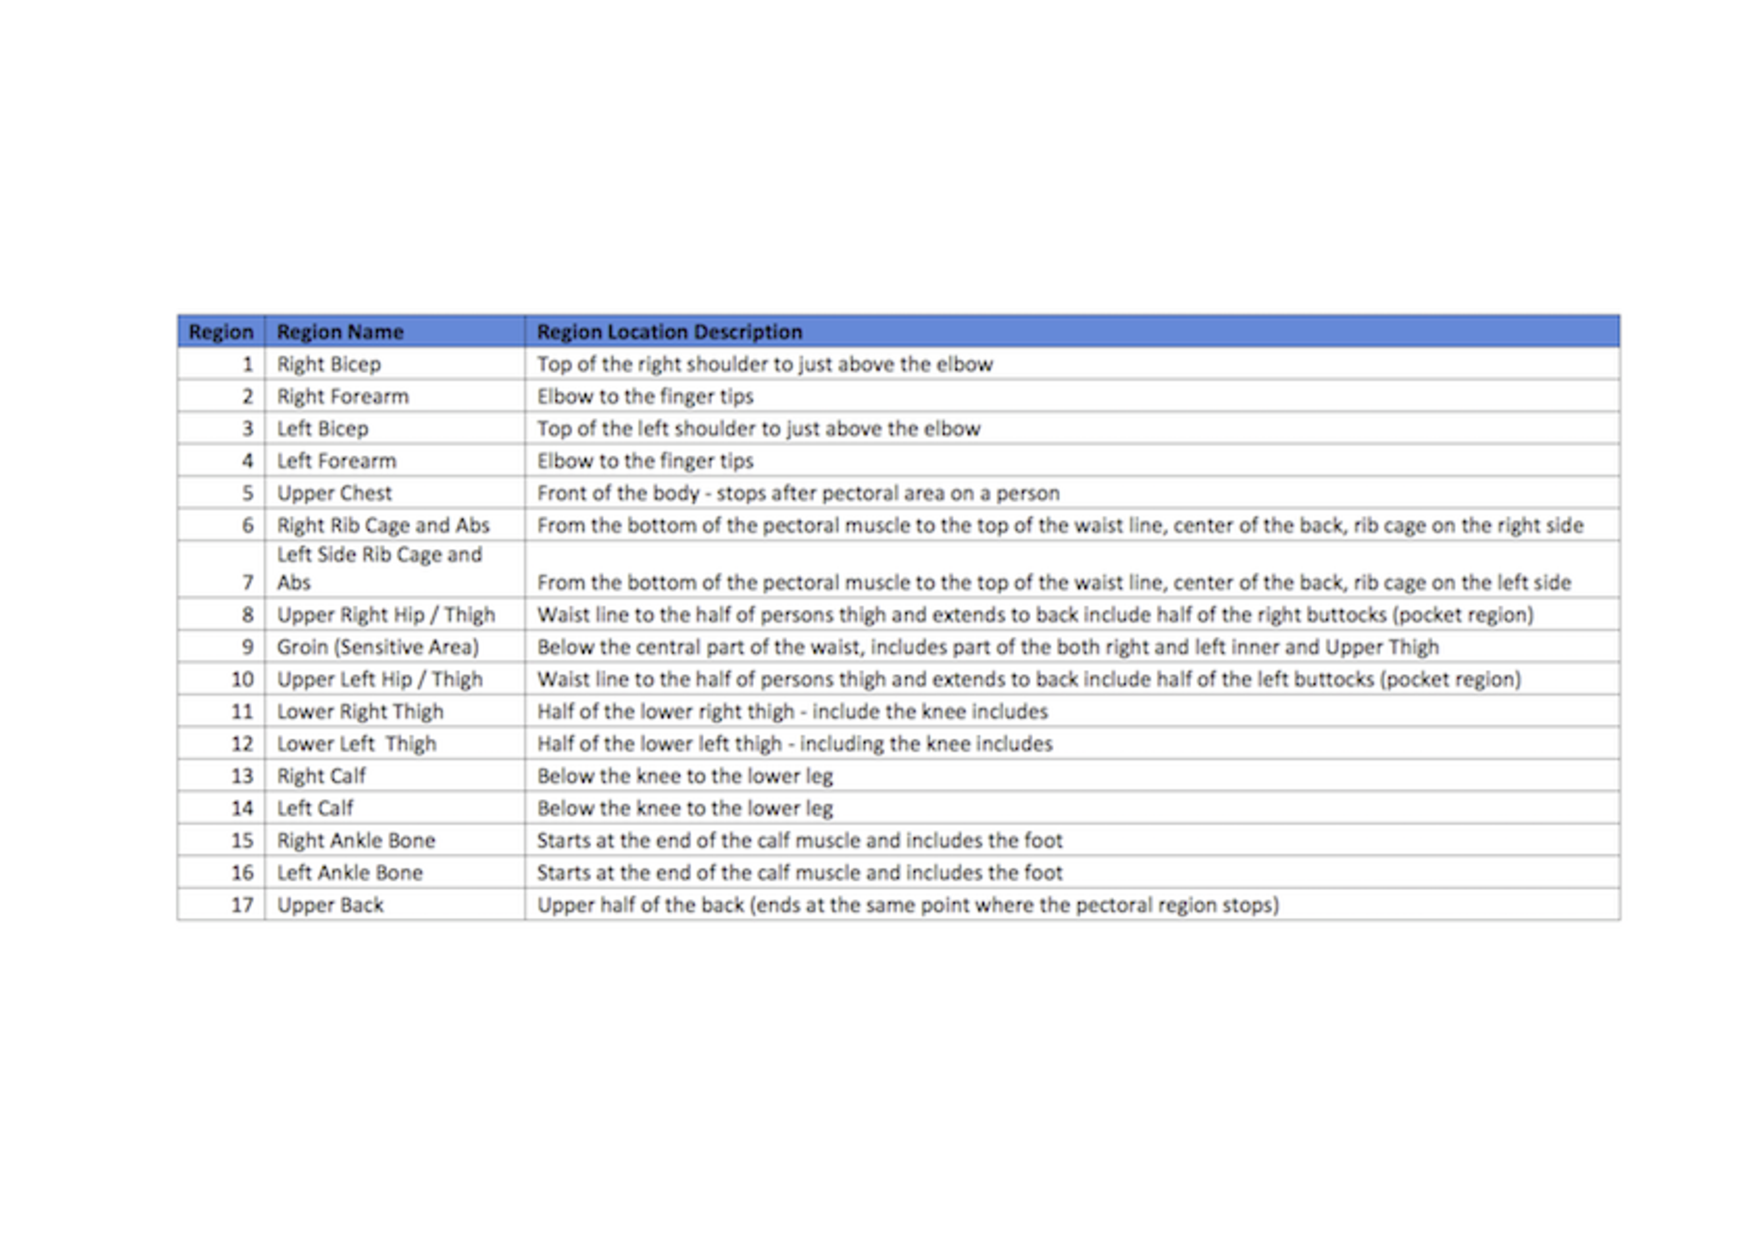
\includegraphics[width=.5\textwidth]{images/body_zones}
\caption{17 regions of a typical human being defined by TSA}
\label{fig:17Region}
\end{figure}

TSA released a set of data containing thousands of packages of images screened by Milli-meter Wave Unit, within each of which there are 16 frames of monochrome images shoot from different perspectives around a single passenger. Each perspective has rotation of 22.5 degrees with respect to the previous one and each image is of size $512\times660$. Moreover, a typical human being in screening process should contain 17 regions as shown in figure~\ref{fig:17Region} with its detailed definitions given in table~\ref{tbl:17Region}. Any potential applicable algorithms should be able to identify any threatening items with respect to these regions. But the problem comes from the provided data: first, there is no or little features and noise is relatively significant; the training is not easy since those labeled data are not well-labeled. Some regions' labels are missed. Plus, the positive labels are of small amount. Out of 1k people and 10k labels, there are only about 1k positive labels; Finally, the computation resource is limited with regard to the dataset. Low resolution images can take 10M per person.

We experimented the sparse representation approach with PCA on cropped regional images, but the result is not ideal. Since there are several regions are occluded from certain perspectives. Inspired by the intrinsic multi-view structure of the provided dataset, we built an Multi-view convolutional network with attention model in order to deal with the regional structure of TSA defined human being.

\begin{table*}[!htb]
\centering
\resizebox{\textwidth}{!}{%
\begin{tabular}{|l|l|l|}
\hline
\multicolumn{1}{|c|}{\textbf{Region}} & \textbf{Region Name} & \textbf{Region Location Description} \\ \hline
1 & Right Bicep & Top of the right shoulder to just above the elbow \\ \hline
2 & Right Forearm & Elbow to the finger tips \\ \hline
3 & Left Bicep & Top of the right shoulder to just above the elbow \\ \hline
4 & Left Forearm & Elbow to the finger tips \\ \hline
5 & Upper Chest & Front of the body \\ \hline
6 & Right Rib Cage and Abs & From the bottom of the pectoral muscle to the top of the waistline, center of the back, rib cage on the right side \\ \hline
7 & Left Rib Cage and Ab & From the bottom of the pectoral muscle to the top of the waistline, center of the back, rib cage on the left side \\ \hline
8 & Upper Right Hip / Thigh & Waistline to the half of person's thigh and extend to back including half of the right buttocks(pocket region) \\ \hline
9 & Groin(Sensitive Area) & Below the central part of the waist, includes part of the both right and left inner and upper thigh \\ \hline
10 & Upper Left Hip / Thigh & Waist line to the half of person's thigh and extend to back including half of the right buttocks(pocket region) \\ \hline
11 & Lower Right Thigh & Half of the lower right thigh - including the knee \\ \hline
12 & Lower Left Thigh & Half of the lower left thigh - including the knee \\ \hline
13 & Right Calf & Below the knee to the lower leg \\ \hline
14 & Left Calf & Below the knee to the lower leg \\ \hline
15 & Right Ankle Bone & Starts at the end of the calf muscle and includes the foot \\ \hline
16 & left Ankle Bone & Starts at the end of the calf muscle and includes the foot \\ \hline
17 & Upper Back & Upper half of the back(ends at the same point where the pectoral region stops) \\ \hline
\end{tabular}%
}
\caption{17 Regions Defined by TSA in Human Screening}
\label{tbl:17Region}
\end{table*}

\begin{figure*}[!t]
\includegraphics[width=\textwidth]{../Pic/finalProject}
\caption{Pipeline}
\label{fig:pipeline}
\end{figure*}
\section{Our Method: MVCNN with LSTM attention}
Figure~\ref{fig:pipeline} presents our pipeline. The core of our algorithm is the MVCNN~\cite{Su_2015_ICCV} with LSTM attention model. Since the We first extend the monochrome image to colored image by filling the other 2 channels with the mean and variance of provided dataset. Then feed these engineered data to our Multi-view CNN, which adopted from the ResNet50 and forward its output to our attention model consisting of ConvNet with kernel size $1\times1$, $3\times3$ and $5\times5$ and an AveragePool. This is for extracting features from different scale. Their output is concatenated and flattened as an sequence, which is later fed to LSTM for quality refinement. The final layer is a fully-connected with output labels on 17 regions per individual image package.

\subsection{Monochrome to Multi-colored Image}
Since the core of our network model is the multi-view CNN, a ResNet50 model, we need 3-channel images as input. Considering naive short-cuts such as replicating the monochrome images or padding blank pixels to the other channels. We instead calculated the mean and variance of the given input images as the blue and green channels, and use the original monochrome image as the red-channel. This alternative provides much more information than the naive inplementations.

\subsection{Network Structure}
After the color-channel engineering, we feed the colored image sequence to the MVCNN. But our task is more tricky since the object may or may not be present, and it can be rather small compared to the human object. Therefore, we proposed to employ Conv-kernel of size $1\times1$, $3\times3$ and $5\times5$ to force the attention of different scale. And then stack their output to feed to the LSTM. The intuition of our attention model is straightforward: 3 convolutions over a same region could gradually report even-detailed information.

\subsection{Stochastic Gradient Descent with Restarts(SGDR)}
The Basic idea of SGDR~\cite{loshchilov2016sgdr} is to restart the learning rate every some time. Learning rate is controlled by a cosine function whose cycle increases each time one cycle concludes. It is reported that the error on CIFAR-10 and CIFAR-100 were 3.14\% and 16.21\% respectively. 
$$ \eta_t = \eta_{min}^i + \frac{1}{2}(\eta_{max}^i-\eta_{min}^i)(1 + \cos(\frac{T_{curr}}{T_i}\pi))$$
$$ T_{i} = T_{i-1} * T_{mult} $$
We set $T_0$, $T_{mult}$ being 100 and 2 respectively. Others the same with the CosineAnnealingLR defined in pytorch

\section{Performance}
[SOME RESULT ANALYSIS AND DIAGRAMS]

\section{Experiment on Sparse Representation using PCA with Image Cropping}
Since the provided data is monochrome and all of them are registered, we naturally came up with the idea of sparse representation. We experiment this idea on regional cropped images.

\subsection{Image Crop}
We have considered the possibility of taking 512*660*16 images as input and a vector of size 17*1 describing the possibility of presence of dangerous objects. However, considering there isn't much positive outcomes, we decided to crop the images and for each zone, only see certain sector of the image.

The image is cropped into 16 sectors, each sector has size 250*250 pixels. The table listed the upper left conner of each sector:
\begin{table}[!htb]
    \centering
    \caption{My caption}
    \label{my-label}
    \begin{tabular}{ccc}
        \hline
        Region \# & x   & y   \\ \hline
        1         & 50  & 50  \\ \hline
        2         & 0   & 0   \\ \hline
        3         & 50  & 250 \\ \hline
        4         & 250 & 0   \\ \hline
        5         & 150 & 150 \\ \hline
        6         & 200 & 100 \\ \hline
        7         & 200 & 150 \\ \hline
        8         & 250 & 50  \\ \hline
        9         & 250 & 150 \\ \hline
        10        & 300 & 200 \\ \hline
        11        & 400 & 100 \\ \hline
        12        & 350 & 200 \\ \hline
        13        & 410 & 0   \\ \hline
        14        & 410 & 200 \\ \hline
        15        & 410 & 0   \\ \hline
        16        & 410 & 200 \\ \hline
    \end{tabular}
    \caption{Region distribution.}
\end{table}
\subsection{Zone assignment}
Now that we have already cropped each image, we will assign each region to it's zones. This makes recognition on each zone easier. Now that no zone can be shown in all 16 images, we will represent it by a None in python.

We have done the pre-calculation to assign sectors based on the index of the image. For example, threat zone 1(Right Bicep) can be see in sector 1 in image 0, 1, 2, 13, 14, 15; in sector 3 in image 6 to 10.

\subsection{Upsample}
For the data set given for now, there are 1871 positive outcomes over 19500 samples, distributed all over 17 zones. This made our work harder because deep learning algorithms will be looking for more positive outcomes to learn. 

We are up sampling the positive outcomes by duplicate positive outcomes and mirror positive images. Thus we will be having more than 5000 positive images. It's unclear whether this is enough.
        
% \section{Conclusion \& Future Works}
% This work presents a 

\bibliographystyle{IEEEtran}
\bibliography{report.bib}
\end{document}
